\documentclass[letter,twocolumn]{article}
\usepackage{tutorial}
\usepackage[OT1]{fontenc}

% ------------------------------------------------------------------------
\usepackage{graphicx}
\usepackage{subfigure}
\usepackage{epsfig}
\usepackage{psfrag}
% used to write c++ code/algorithms
\usepackage{listings}
\usepackage{fancyvrb}

%\psdraft

\twocolumn


% hyperref stuff
\usepackage{hyperref}
\hypersetup{
  pdftitle={A Tutorial on CGAL Polyhedron for Subdivision Algorithms},
  pdfauthor={INRIA Geometrica},
  pdfsubject={A tutorial for CGAL},
  pdfkeywords={},
  pdfpagemode=UseThumbs,
  baseurl={http://www.cgal.org},
  colorlinks=true,
  linkcolor=black,
  anchorcolor=black,
  citecolor=black,
  filecolor=black,
  menucolor=black,
  pagecolor=black,
  urlcolor=blue,
  bookmarksopen=false,}
% end hyperref stuff

\lstset{language=C++, basicstyle=\scriptsize}

\graphicspath{{figs/}}
\def\figurename{Figure}
\def\tablename{Tableau}
\newcommand{\italic}[1]{\emph{#1}} 

% ------------------------------------------------------------------------
\newcommand\IL{{\itshape left}}
\newcommand\IR{{\itshape right}}
\newcommand\IM{{\itshape middle}}
\newcommand\IT{{\itshape top}}
\newcommand\IB{{\itshape bottom}}

% ------------------------------------------------------------------------
\newcommand{\CodeFmt}[1]{{\small\texttt{#1}}}

\def\kernel{\CodeFmt{Kernel}}

\def\cgalpoly{\CodeFmt{CGAL::Polyhedron\_3}}
\def\poly{\CodeFmt{Polyhedron\_3}}
\def\polytrait{\CodeFmt{PolyhedronTraits\_3}}
\def\polyitem{\CodeFmt{PolyhedronItems\_3}}
\def\polybuilder{\CodeFmt{Polyhedron\_incremental\_builder\_3}}

\def\cgalhds{\CodeFmt{CGAL::HalfedgeDS}}
\def\hds{\CodeFmt{HalfedgeDS}}
\def\hdsitem{\CodeFmt{PolyhedronItems}}

% L.K. -------------------------------------------------------------------
\newcommand{\CC}{C\raise.08ex\hbox{\texttt{++}}}
\newcommand{\openmesh}{\textsc{OpenMesh}}
\newcommand{\opensg}{\textsc{OpenSG}}
\newcommand{\cgal}{\textsc{Cgal}}
\newcommand{\stl}{\textsc{Stl}}


% =========================================================================
\begin{document}

% TITLE
% ------------------------------------------------------------------------
\date{}
\title{{\LARGE {\sffamily\bfseries A Tutorial on CGAL Polyhedron \\
                                   for Subdivision Algorithms}}}


\author{\small
\sffamily Le-Jeng Shiue\footnote{SurfLab, University of Florida}
\and \small
\sffamily Pierre Alliez\footnote{GEOMETRICA, INRIA Sophia-Antipolis}
\and \small
\sffamily Radu Ursu\footnote{Geometry Factory, Sophia-Antipolis}
\and \small
\sffamily Lutz Kettner\footnote{MPII, Saarbr\"ucken}}
\maketitle

\thispagestyle{empty}

{\scriptsize
This document is the abstract of the tutorial on CGAL
polyhedron for subdivision algorithms. The complete 
version of the tutorial and the accompanied sorce code 
can be downloaded at [...].
}

% ------------------------------------------------------------------------
\subsection*{Introduction}

A tutorial on the CGAL polyhedron data structure
is presented assuming familiarity with the \CC\ 
template mechanism and the key concepts of the generic 
programming. The tutorial is organized around
subdivision surfaces in a polyhedron viewer.
The polyhedron viewer (Figure \ref{viewer}) demonstrates the
basic functionalities of the \cgalpoly\ and some extended
functionalities such as file I/O, mesh superimposition, and trackball
manipulation. Several subdivision surfaces are supported
in the polyhedron viewer, including Catmull-Clark, Loop, 
Doo-Sabin, $\sqrt{3}$ and Quad-Triangle subdivisions. 
The tutorial shows how to implement subdivision
surfaces in two different mechanisms provided by \cgalpoly :
\emph{Euler operators} and \emph{modifier callback mechanism}. 
A $\sqrt{3}$ subdivision implementation is designed based on the
Euler operators and a Quad-Triangle subdivision implementation
is designed based on overloading the modifier.  
Extened from the previous design, a 
\emph{combinatorial subdivision library} (CSL) is
then proposed with the increased sophistication and 
abstraction. CSL abstracts the geometry operations from 
the refinements. Subdivisions in CSL is structured as a 
combination of a refinement host and the template geometry 
policies. With several fundanmental refinement schemes in stock,
CSL is established by specilaizing the refinements with a set of 
user-defined geometry policies.

\begin{figure}[htb]
  \centering
  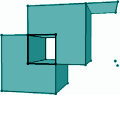
\includegraphics[width=\linewidth]{figs/teaser}\\ {\scriptsize Demo
  application running on Windows. A coarse polygon mesh is subdivided
  using the quad-triangle subdivision scheme.}
  \label{fig:viewer}
\end{figure}


% ------------------------------------------------------------------------
\subsubsection*{CGAL Polyhedron}

Polyhedron data structures based on the concept of halfedges have been
very successful for the design of general algorithms on meshes.
Although making a preliminary version of a halfedge-based mesh data
structure (HDS) is as a fairly simple task and is often proposed as a
programming exercise, there now exists a general purpose HDS available
which is worth considering relying on. With the successful use of
generic programming in \CC , a set of reusable library components for
graphics modeling and geometry processing are demanded by researchers
and developers. \italic{Extensible algorithm} models based on a
\italic{robust, efficient and customizable polyhedron data structure}
will certainly speed up the research as well as the development cycle,
and benefit the community of geometric computing and geometry
processing.

Most mesh algorithms employ a customized halfedge data structures and
most of the customizations are specialized by customizing the
primitive data, which are the vertex positions, the facet normals or
other data used for algorithmic purposes. \cgalpoly\ encapsulates a
generic design of the halfedge data structure allowing users customize
the \poly\ with the template parameters of the geometry
primitives. There are several advantages employing the \poly\ as the
core data structure of a mesh processing application: \\

\indent $\bullet$ The \poly\ is a \italic{generic} data structure.\\
\indent $\bullet$ The \poly\ is a \italic{robust} and \italic{optimized} 
                  data structure.\\
\indent $\bullet$ A complete set of geometric entities and predicates
                  is provided within CGAL.\\
\indent $\bullet$ CGAL is closely following the programming 
                  style of the \CC\ STL.




% ------------------------------------------------------------------------
\subsection*{Tutorial Outlines}

% ------------------------------------------------------------------------
\subsubsection*{Polyhedron Viewer}

%% We have designed and implemented an application based on the
%% \cgalpoly. This program provides a polyhedron viewer of
%% following functionalities:\\
%% \indent $\bullet$ File I/O,\\
%% \indent $\bullet$ polyhedron rendering,\\ 
%% \indent $\bullet$ and trackball manipulation.\\
%% In addition to these built-in functions, the viewer is accompanied
%% with a set of subdivision algorithms that generate smooth polyhedron
%% surfaces from a coarse polyhedron. \italic{The tutorial instructs the
%% readers through the design and the implementation of the polyhedron
%% viewer and the subdivisions}. The first part of the tutorial
%% highlights the design and implementation issues related to the \poly\
%% used in the viewer. The second part of the tutorial explains how to
%% implement the connectivity and geometry operations of the subdivision
%% algorithms. The source codes are going to be published with the
%% releasing of the tutorial.

The tutorial starts with demonstrating how to implement a simple
viewer based on the default configuration of the \cgalpoly . This
simple viewer demonstrates some basic functionalities of the
\cgalpoly\ such as \italic{modifier} and \italic{incremental builder} 
for initialization and the mesh traversal, i.e. the \italic{iterators}
and the \italic{circulators}, for rendering or mesh exporting. Based
on this simple viewer, we then show the readers how to
\italic{customize the \poly} to support certain functionalities. 
An enriched polyhedron is proposed with the primitives specialized
with algorithmic flags. This enriched polyhedron is used as the core
data structure of our application.  We then show how to interact with
a customized \poly.  The extended primitives are employed to support
the superimposition of the input mesh on the subdivided surfaces. A
trackball function of the enriched polyhedron is also demonstrated in
the tutorial.

% ------------------------------------------------------------------------
\subsubsection*{Subdivision Algorithms}

The second part of the tutorial focuses on the design and the
implementation of $\sqrt{3}$ subdivision (Figure \ref{fig:sqrt3}) 
and Quad-Triangle subdivision (Figure \ref{fig:quad-triangle}).  

\begin{figure}[htb]
    \centering{\includegraphics[width=7.0cm]{figs/sqrt3}}
    \caption{$\sqrt{3}$ subdivision of the mannequin mesh.}
    \label{fig:sqrt3}
    \vspace{0.5cm}
    \centering{\includegraphics[width=7.0cm]{figs/quad-triangle}}
    \caption{Quad-Triangle subdivision of the rhombicuboctahedron mesh.}
    \label{fig:quad-triangle}
\end{figure}

In addition to its importance in the surface modeling, we 
choose subdivision algorithms to demonstrate both the 
\italic{topology operation} (refinement) and the
\italic{geometry operations} (smoothing) of a
CGAL Polyhedron. 
%The topology and the geometry
%operations are the two basic operations required by most geometry
%algorithms. 
The key to implement a subdivision algorithm is to effficiently support
the refinement, i.e.\ the connectivity modifications. Two approaches
are introduced to support the refinement: the \italic{
Euler operators} (operator scheme) and
the \italic{modifier callback mechanism} (modifier scheme). 
The operator scheme reconfigures the connectivity with a 
combination of Euler operators. $\sqrt{3}$ subdivision~\cite{sqrt3} is
used to demonstrate this scheme. Though simple and efficient in some
refinements, e.g.\ $\sqrt{3}$ subdivision, the correct combination of
the operators is hard to find for some refinements, e.g.\ Doo-Sabin
subdivision~\cite{ds}. The modifier scheme solves the problem by
letting the programmers create their own combinatorial operators 
using the polyhedron incremental builder. Quad-Triangle
subdivision~\cite{qts,l-pg-03} is used to demonstrate this scheme.


% ------------------------------------------------------------------------
\subsubsection*{Combinatorial Subdivision Library}

A \emph{C}ombinatorial \emph{S}ubdivision \emph{L}ibrary 
(CSL) is designed based on the policy-based design 
\cite{Alexandrescu:2001:MCD}.
The policy-based design assembles a class
(called \emph{host}) with complex behavior out of many 
small behaviors (called \emph{policies}).
Each policy defines an interface for a
specific behavior. CSL proposes a 
generic subdivision solution as a \emph{refinement function}
parameterized with the \emph{smoothing rules}.
The refinement function refines the control mesh,
maintains the correspondence between the control mesh and refined
mesh, and applies the smoothing stencils provided by the policy
class. For example, Catmull-Clark subdivision~\cite{cc} is structured
as a quadralization function parameterized with the Catmull-Clark
smoothing rules.
\begin{lstlisting}
void CatmullClark_subdivision(Polyhedron& p) {    
  quadralize_polyhedron<CatmullClark_rule<Polyhedron>>(p);  
}
class CatmullClark_rule {
public:
  void facet_rule(  Facet_handle  facet, Point& pt);
  void edge_rule(Halfedge_handle   edge, Point& pt);
  void vertex_rule(Vertex_handle vertex, Point& pt);
};
\end{lstlisting}

\noindent The \CodeFmt{quadralize\_polyhedron<>()} 
is the host function refining the input mesh
and the \CodeFmt{CatmullClark\_rule} is the policy 
class applying the Catmull-Clark stencils.
This approach offers a convenient way to
specialize a subdivision with the template smoothing rules.
CSL currently supports Catmull-Clark~\cite{cc}, 
Loop~\cite{loop} and Doo-Sabin~\cite{ds} subdivisions.
CSL accepts a polyhedron mesh specialized from the
\cgalpoly .  
%not just the enriched polyhedron we used in the polyhedron
%viewer. 


% ------------------------------------------------------------------------
\subsection*{Intended Audience}

The intended audience of the tutorial are researchers, developers or
students developing algorithms around meshes. Experience in advanced
\CC\ design (i.e.\ generic programming using templates) and knowledge
of the halfedge data structure and subdivisions are prerequisites.

% references
{\footnotesize
\bibliographystyle{alpha}
\bibliography{abstract}
}

\end{document}
